\section{Situación Actual}

En la actualidad podemos encontrar diversos intentos de modernizar los procesos administrativos de entidades públicas y podemos tomar sus experiencias como inspiración para la realización de una herramienta reutilizable de software. Además, existen paquetes de software que, aunque de manera indirecta, pueden ayudar en la creación de trámites.
\subsection{Normativa relevante}
\subsubsection{Gobierno Electrónico y su normativa}
Cuando hablamos de Gobierno Electrónico y su normativa es menester citar a la Constitución Política del Estado Plurinacional de Bolivia, misma que en su Art. 103 y 298 denota la importancia del desarrollo de la ciencia y la investigación a favor de las bolivianas y los bolivianos. Además, reconoce como prioridad el uso de las tecnologías y comunicación para el vivir bien. Al respecto el Artículo 103 establece lo siguiente:"I. El Estado garantizará el desarrollo de la ciencia y la investigación científica, técnica y tecnológica en beneficio del interés general. Se destinarán los recursos necesarios y se creará el sistema estatal de ciencia y tecnología. II. El Estado asumirá como política la implementación de estrategias para incorporar el conocimiento y aplicación de nuevas tecnologías de información y comunicación. III. El Estado, las universidades, las empresas productivas y de servicio públicas y privadas, y las naciones y pueblos indígena originario campesinos, desarrollarán y coordinarán procesos de investigación, innovación, promoción, divulgación, aplicación y transferencia de ciencia y tecnología para fortalecer la base productiva e impulsar el desarrollo integral de la sociedad, de acuerdo con la ley." Asimismo el Artículo 298 de la citada normativa legal en su parte pertinente establece lo siguiente: "(...)II. Declara prioridad nacional la promoción del uso de las tecnologías de información y comunicación para procurar el vivir bien de todas las bolivianos y bolivianos. (...)"
A su vez es menester citar la Ley N°164 - Ley General de Comunicaciones, Tecnologías de Información y Comunicación, misma que en su Artículo 71 declara prioridad nacional la promoción y uso de tecnologías de información y comunicación para procurar el vivir bien de todas las bolivianas y bolivianos. Por otra parte, el párrafo I del el Artículo 72 de la citada noma legal, establece el rol de Estado con referencia al uso de las TIC´S, el despliegue y uso de infraestructura, el desarrollo de contenidos y aplicaciones, la protección de las usuarias y usuarios, la seguridad informática y redes como mecanismos de democratización de oportunidades para todos los sectores de la sociedad y especialmente para aquellos con menores ingresos y con necesidades especiales, a su vez el Artículo 75 de la citada norma legal, hace referencia a Gobierno Electrónico, mismo que establece de forma expresa lo siguiente: "I. El nivel central del Estado promueve la incorporación del Gobierno Electrónico a los procedimientos gubernamentales, a la prestación de sus servicios y a la difusión de información, mediante una estrategia enfocada al servicio de la población. II. El Órgano Ejecutivo del nivel central del Estado, elaborará los lineamientos para la incorporación del Gobierno Electrónico." Asimismo el Artículo 76, define el Alcance de Gobierno Electrónico, mismo que señala lo siguiente: "(...) El Estado fijará los mecanismos y condiciones que las entidades públicas aplicarán para garantizar el máximo aprovechamiento de las tecnologías de la información y comunicación, que permitan lograr la prestación de servicios eficientes." 
 Otra normativa que regula lo referente al Gobierno Electrónico, se puede citar al Reglamento para el Desarrollo de Tecnologías de Información y Comunicación - Decreto Supremo N° 1793, mismo que en su Art. 17 establece el objetivo de Gobierno Electrónico, señalando lo siguiente: "(...)I. Modernizar y transparentar la gestión pública, otorgando servicios y atención de calidad a la ciudadanía, garantizando el derecho a la información, así como contribuir a la eficiencia y eficacia de los actos administrativos en los procesos internos del gobierno, mediante el uso de las tecnologías de información y comunicación y otras herramientas. II. Generar mecanismos tecnológicos de participación y control social, mediante el uso de TIC por parte de los ciudadanos, organizaciones sociales y pueblos y naciones indígena originario campesinos."
\subsubsection{Software Libre y su regulacioón normativa}
\subsubsection{Soberania Digital y las leyes}
\subsubsection{El trámite administrativo y su regulación normativa}
Al respecto cuando hablamos de la regulación normativa del tramite administrativo es menester citar al Decreto Supremo N°3525, el cual en su art. 12 establece lo siguiente:"Artículo 12°.- (Trámites administrativos) I. Las instituciones públicas deberán priorizar en todos sus trámites el uso de tecnologías de información y comunicación a efecto de digitalizar, automatizar, interoperar y simplificar la tramitación de los asuntos que son de su competencia. II. Para facilitar la realización de trámites a la ciudadanía, las entidades públicas, en observancia de su normativa específica, deberán intercambiar entre ellas datos e información mediante interoperabilidad. Los mecanismos y condiciones de publicación y acceso a los servicios de interoperabilidad serán establecidos por el Ente Rector de Gobierno Electrónico y Tecnologías de Información y Comunicación. III. El intercambio de datos e información mediante interoperabilidad no afectará la percepción de recursos de las entidades públicas titulares de la información por la prestación del servicio público. IV. Las entidades públicas no podrán exigir al administrado como requisito ningún documento que hubiera sido emitido por la misma entidad, o cuya información esté disponible mediante servicios de interoperabilidad de otra entidad. V. Las entidades públicas no podrán exigir al administrado como requisito ningún documento que hubiera sido requerido con anterioridad, salvo actualización o modificación y conforme a normativa legal vigente. VI. Las entidades públicas tendrán un plazo máximo de veinte (20) días hábiles a partir de la publicación de un nuevo servicio de interoperabilidad para adecuar sus procesos y procedimientos al mismo" A su vez el Art. 13 del citado decreto establece lo siguiente: "Artículo 13°.- (Entidades generadoras de información) I. Las entidades que conforme a sus atribuciones recolectan, generan, transforman y validan datos o información, son responsables en observancia de su normativa legal específica, de publicar la información y datos como fuente primaria a través de la plataforma de interoperabilidad establecida en el Plan de Implementación de Gobierno Electrónico aprobado mediante el Decreto Supremo Nº 3251, de 12 de julio de 2017. II. En el marco de procesos de actualización, certificación o emisión de copias legalizadas de documentos que aún se encuentren en formato físico, los datos e información pertinente consignados en los mismos deberán ser registrados en medios digitales que permitan ser publicados mediante servicios de interoperabilidad.(...)"
\subsection{Sistemas realizados para el control de trámites}

Sólo en Latinoamérica, cada país reportó mediante las autoridades de gobierno electrónico tener entre 1000 y 5000 trámites diferentes. Esto implica que ya hubo muchos esfuerzos para crear sistemas que digitalicen esta actividad. A continuación se listan algunos.

\subsubsection{A nivel académico}

Podemos encontrar una gran cantidad de proyectos de grado realizados en la región que tratan sobre la implementación de sistemas de control de trámites:

\begin{itemize}
    \item SISTEMA DE CONTROL DE TRÁMITES UTILIZANDO MAQUINAS DE TURING CASO: DIVISIÓN DE GESTIONES ADMISIONES Y REGISTROS U.M.S.A.
    \item Desarrollo e Implementación del Sistema de Tramite
          Documentario en la Municipalidad Provincial de
          Huancayo para la atencion de expedientes.
    \item DESARROLLO DE UN SISTEMA WEB PARA MEJORAR  EL PROCESO DE TRÁMITE DOCUMENTARIO ADMINISTRATIVO DEL HOSPITAL SUB REGIONAL DE  ANDAHUAYLAS
    \item Sistema de información de trámite documentario basado en tecnología web para institutos de educación superior tecnológicos de la región Ancash en el año 2016
    \item Programa de automatización de los procedimientos de trámite documentario en la calidad del servicio a los usuarios del Hospital Nacional Arzobispo Loayza – Lima, 2016
    \item Implementación de un sistema de trámite documentario para la Agencia de Compras de las Fuerzas Armadas
    \item Implementación De Un Módulo De Control Y Seguimiento Para Mejorar La Gestión Del Trámite Documentario En La Municipalidad Distrital De Cayaltí, 2018
    \item Desarrollo de una aplicación \textit{web responsive} para mejorar el proceso de trámite documentario en un colegio profesional
    \item Desarrollar un sistema web de trámite documental para mantener las acreditadoras de la escuela de ingeniería informática de la URP
\end{itemize}

De estos trabajos podemos destacar dos por su relevancia con el proyecto que se propone en este documento:

\paragraph{SISTEMA DE CONTROL DE TRÁMITES UTILIZANDO MAQUINAS DE TURING CASO: DIVISIÓN DE GESTIONES ADMISIONES Y REGISTROS U.M.S.A.}

En este proyecto de grado, realizado el año 2007, se toma como enfoque teórico a las máquinas de Turing. En dichas máquinas, que son un modelo matemático de computación, se describe una suerte de cinta dividida en casillas que funciona como memoria y un cabezal que escribe y lee de esa cinta, cambiando de estados. Esta conceptualización, sin ser estrictamente especificada se puede ver repetida en otras implementaciones de módulos de control de trámites.

\paragraph{Implementación De Un Módulo De Control Y Seguimiento Para Mejorar La Gestión Del Trámite Documentario En La Municipalidad Distrital De Cayaltí}

Esta tesis busca demostrar la importancia de la creación de un módulo específico de trámites que sea reutilizable. Brinda algunas recomendaciones sobre su implementación, pero no realiza ninguna implementación práctica.

\subsubsection{A nivel comercial}

Si bien, no existen módulos de trámite que se puedan integrar en sistemas más grandes de manera comercial, sí se puede ver sistemas completos con la funcionalidad de gestión de trámites que ofrecen todo lo necesario para llevar a cabo procesos administrativos. Algunos son:

\begin{itemize}
    \item \textit{SoftExpert} - Gestión de Trámites: Visibilidad y control sobre el procesamiento de documentos, archivos y objetos
    \item R2 Docuo: Expedientes, Solicitudes y trámites a toda velocidad: En su \textit{homepage} puede verse la funcionalidad de seguimiento temporal de trámites (figura \ref{fig:r2docuotimeline})
    \item \textit{Filestage}: Si bien no es específico para trámites, tiene un sistema de tránsito de documentos hasta su aceptación, que es una funcionalidad común en los trámites.
\end{itemize}

\begin{figure}[!htpb]
    \centering
    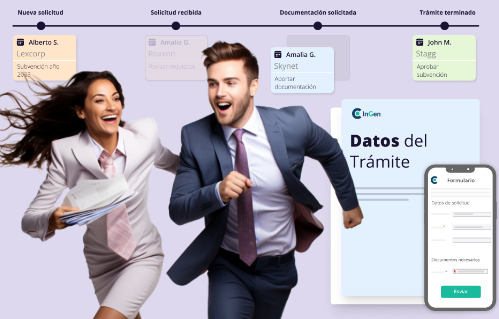
\includegraphics[width=0.7\textwidth]{assets/r2docuotimeline}
    \caption{Captura del homepage de R2 Docuo donde se puede ver el timeline de un trámite}{Fuente: https://www.r2docuo.com/es/expedientes-y-tramites}
    \label{fig:r2docuotimeline}
\end{figure}

Se debe notar que si bien los dos primeros logran la funcionalidad deseada en este proyecto, no permiten la personalización, no son necesariamente software libre y no se pueden introducir en sistemas más grandes de la misma manera que lo haría un paquete de software reutilizable.

\subsection{Paquetes de software que facilitan la creación de módulos de trámites}

La cantidad de paquetes de software que existen y que se puede considerar que ayudan en el proceso de gestión, control y seguimiento de trámites es abundante, por lo que nos centraremos en aquellas presentes en el ecosistema de \textit{Laravel}.

El seguimiento de trámites requiere que tengamos guardada la información de todos los pasos de un trámite y los cambios realizados. Además, la naturaleza de los trámites, como se podrá ver en el análisis de la solución, tiene que ver con estados (pasos de un procedimiento administrativo). Es por esto que las siguientes librerías podrían ser utilizadas con un objetivo similar al paquete que se pretende desarrollar en este proyecto:

\begin{itemize}
    \item \textit{Laravel Auditing}: Permite mantener control sobre los datos en una aplicación y para hacer seguimiento de los cambios realizados en los mismos. Es muy potente y fácil de usar.
    \item \textit{Laravel Eloquent State Machines}: Máquinas de estado aplicadas sobre los modelos \textit{Eloquent} (figura \ref{fig:laravelstatemachines}).
    \item \textit{Laravel-Permission}: Permite asociar usuarios con roles.
\end{itemize}

\begin{figure}[!htpb]
    \centering
    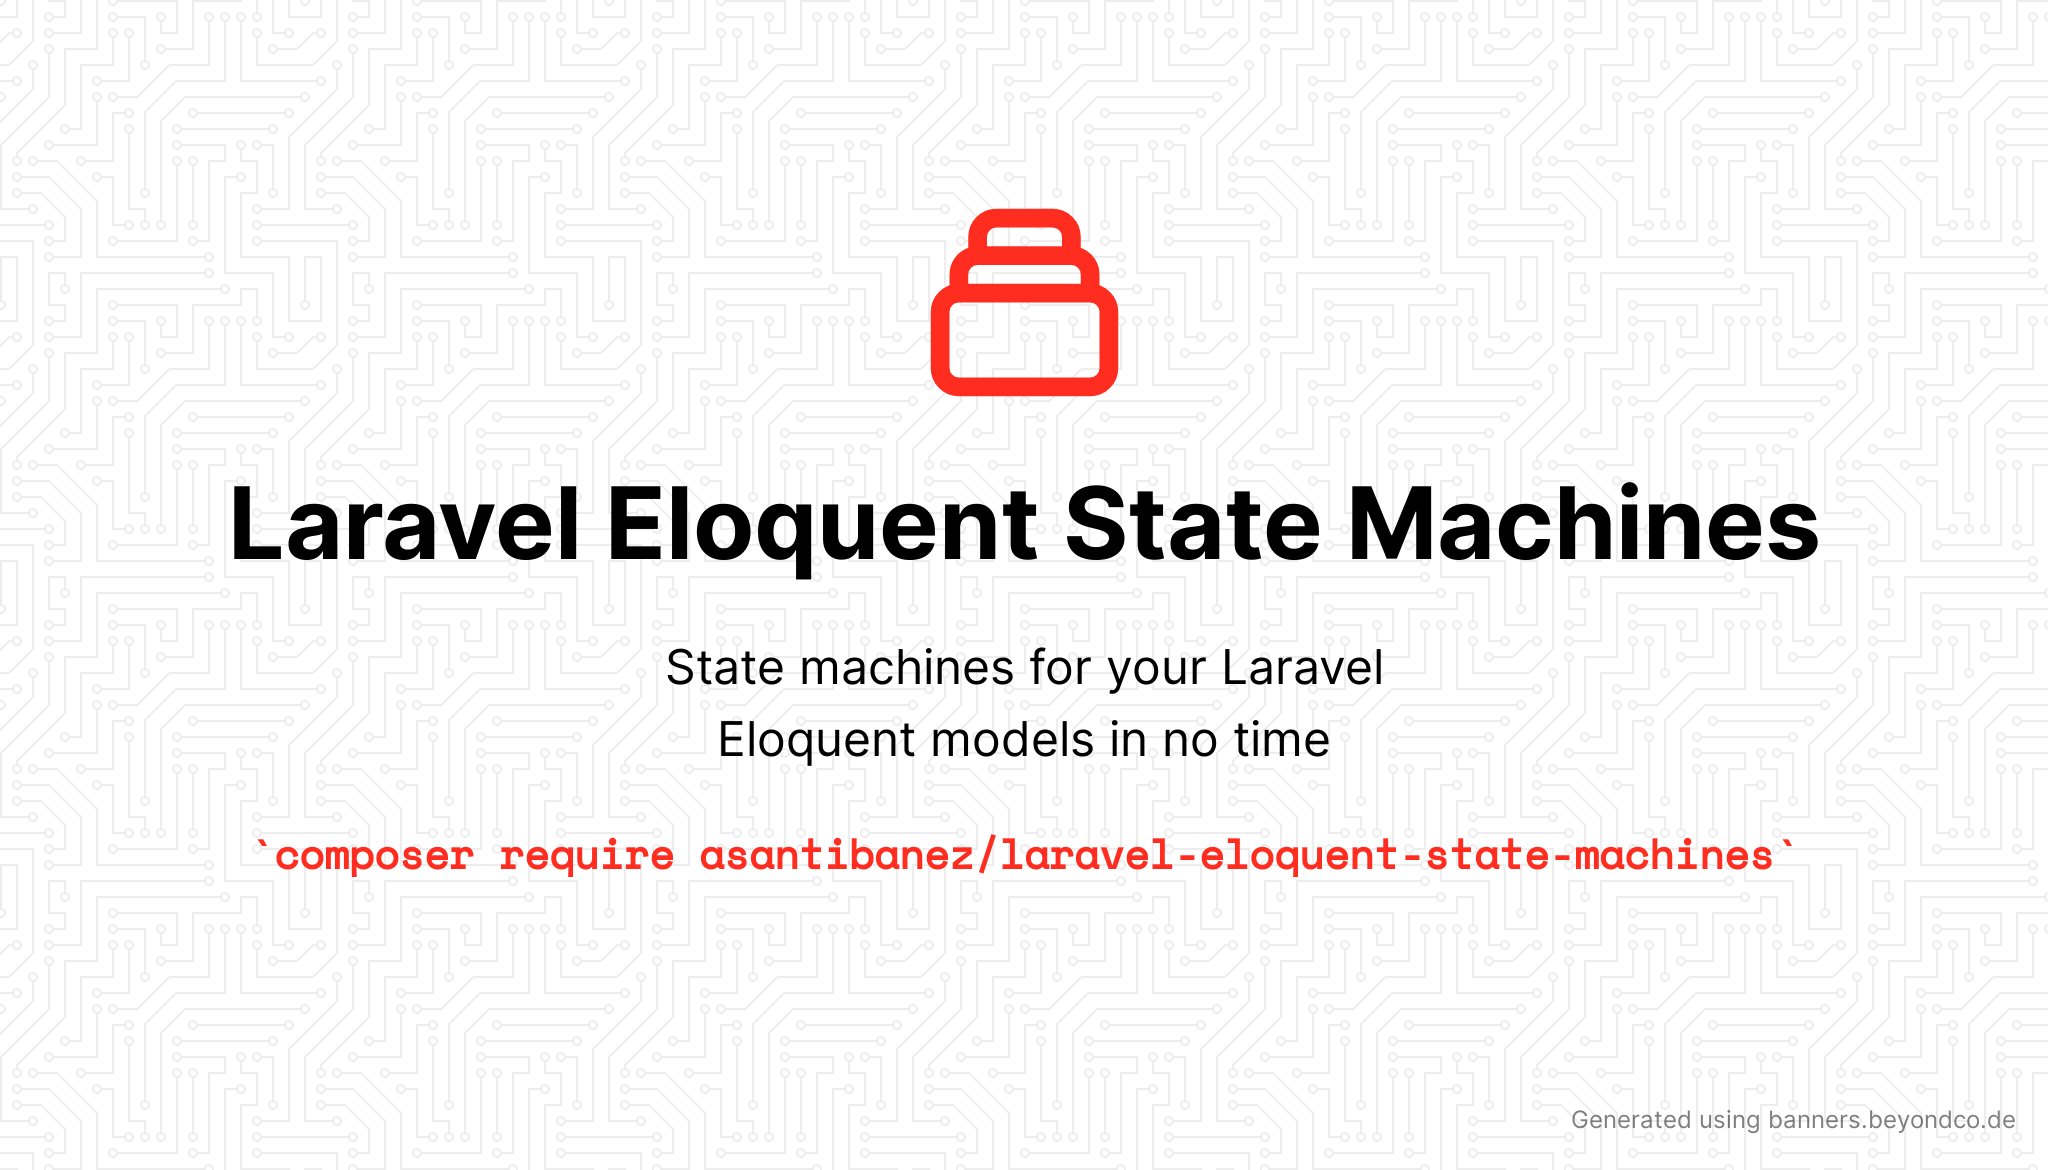
\includegraphics[width=0.7\textwidth]{assets/laravelstatemachines}
    \caption{Paquete de manejo de estados en Laravel}{Fuente: https://github.com/asantibanez/laravel-eloquent-state-machines}
    \label{fig:laravelstatemachines}
\end{figure}

De los tres paquetes anteriores, sin duda el de las máquinas de estados es el que más inspirará este proyecto. La funcionalidad es similar a la que se pretende, pero no es específica a los procesos administrativos y por lo tanto no brinda ciertas herramientas que podrían ser necesarias en los mismos, como el seguimiento, el cual podría ser implementado con la ayuda del segundo paquete mencionado.
